\documentclass[onecolumn, draftclsnofoot, 10pt, compsoc]{IEEEtran}
\usepackage{graphicx}
\usepackage{url}
\usepackage{setspace}
\usepackage{hyperref}
\usepackage{indentfirst}
\usepackage{geometry}
\geometry{textheight=9.5in, textwidth=7in}

% 1. Fill in these details
\def \CapstoneTeamName{		Team Ancestry Data Viewer(ADVR)}
\def \CapstoneTeamNumber{		22}
\def \GroupMemberOne{			YongPing Li}
\def \GroupMemberTwo{			Monica Sek}
\def \GroupMemberThree{			Le-Chuan Chang}
\def \CapstoneProjectName{		Ancestry Data Viewer}
\def \CapstoneSponsorCompany{	}
\def \CapstoneSponsorPerson{		Ashley McGrath}

% 2. Uncomment the appropriate line below so that the document type works
\def \DocType{	%Problem Statement
				%Requirements Document
				%Technology Review
				%Design Document
				Progress Report
				}
			
\newcommand{\NameSigPair}[1]{\par
\makebox[2.75in][r]{#1} \hfil 	\makebox[3.25in]{\makebox[2.25in]{\hrulefill} \hfill		\makebox[.75in]{\hrulefill}}
\par\vspace{-12pt} \textit{\tiny\noindent
\makebox[2.75in]{} \hfil		\makebox[3.25in]{\makebox[2.25in][r]{Signature} \hfill	\makebox[.75in][r]{Date}}}}
% 3. If the document is not to be signed, uncomment the RENEWcommand below
%\renewcommand{\NameSigPair}[1]{#1}

%%%%%%%%%%%%%%%%%%%%%%%%%%%%%%%%%%%%%%%
\begin{document}
\begin{titlepage}
    \pagenumbering{gobble}
    \begin{singlespace}
    	
\includegraphics[height=4cm]{coe_v_spot1}
        \hfill 
        % 4. If you have a logo, use this includegraphics command to put it on the coversheet.
        %\includegraphics[height=4cm]{CompanyLogo}   
        \par\vspace{.2in}
        \centering
        \scshape{
            \huge CS Capstone \DocType \par
            {\large\today}\par
            \vspace{.5in}
            \textbf{\Huge\CapstoneProjectName}\par
            \vfill
            {\large Prepared for}\par
            \Huge \CapstoneSponsorCompany\par
            \vspace{5pt}
            {\Large\NameSigPair{\CapstoneSponsorPerson}\par}
            {\large Prepared by }\par
            Group\CapstoneTeamNumber\par
            % 5. comment out the line below this one if you do not wish to name your team
            \CapstoneTeamName\par 
            \vspace{5pt}
            {\Large
                \NameSigPair{\GroupMemberOne}\par
                \NameSigPair{\GroupMemberTwo}\par
                \NameSigPair{\GroupMemberThree}\par
            }
            \vspace{20pt}
        }
        \begin{abstract}
        % 6. Fill in your abstract    
This document is a report on how much progress has been made on the development of the Ancestral Data Viewer application. This document also identifies problems that have delayed progress, and solutions or potential solutions to those problems.
        \end{abstract}     
    \end{singlespace}
\end{titlepage}
\newpage
\pagenumbering{arabic}
%\tableofcontents
% 7. uncomment this (if applicable). Consider adding a page break.
%\listoffigures
%\listoftables
\clearpage

% 8. now you write!
\section{Introduction }
\begin{singlespace}
The purpose of our project is to read GEDCOM files, because they are very difficult to read and cluttered with information. The goal is to create an ancestry data viewer software that is capable of displaying the information onto an ancestry tree. The software first parses the GEDCOM file to get the information. The information is then organized with the display algorithm. The UI should also be implemented to allow the users to interact with the software. The software also needs to be capable of displaying the ancestry tree with multiple views: 2D, 3D, and lineage. Therefore, the software needs to able to detect whether if a VR device is connected and if so, change to 3D view for 3D view, and for the direct lineage view, we need to be able to find the ancestor and descendants of a given person.
\end{singlespace}

\section{Yong Ping Li}
\begin{singlespace}
Currently on the project, I have implemented the parser which can be considered finished but we still need to manipulate the information we parsed to make it more easily accessed. For implementing the parser, I first search and download examples of GEDCOM file. From there, I analyze the structure of the GEDCOM files. The GEDCOM file first starts off with some information about the family, and then lots of tags that we do not need, and information about individuals after that. There are two pieces of information that we need from the individual's section and that is some form of identification and their name. Identification is needed because we might have people with the same names in the family. We need to able to distinguish each individual person from others. Identification for individuals already exist in the GEDCOM file, and we don't have to create our own. As I went through the GEDCOM file, I found tags that I didn't know what meaning of and I went online and did more research. I found a website with detailed information about each tag in the GEDCOM file and successfully identify all the information as well as the tags corresponding to each type of information. The parser was implemented after figuring out the corresponding tags and it is capable of gathering all the needed information. The image below is an example of what the parsed information that I printed into a file. There is more information on the right displaying the children of each person if they have any.
\newline
\newline
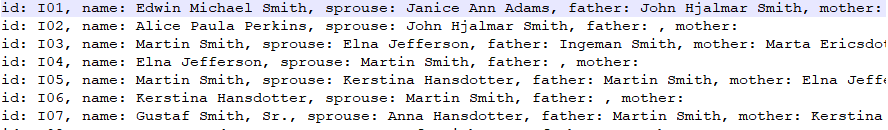
\includegraphics[height=5cm,width=18cm]{data}\\
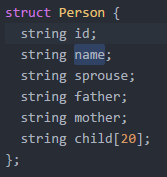
\includegraphics[height=5cm]{struct}
\newline
The information gathered is stored in a struct array. The struct array contains six variables and that is id, name, Spouse, father, mother, and child(image above)It is storing information about the individual and names of people who are directly related to the individual. Therefore, the individuals are somewhat linked together, but there are problems with doing it this way. First of all, there can be duplicate names in the family which will cause the functions within our parser to get the wrong information. If we change the fields from storing names to storing the identification of individuals could fix this problem but it makes names of individuals more difficult to access. Therefore, I will start implementing the tree structure for storing the information which is more easier to access. I have implemented a function inside the parser to find the root nodes of the ancestry tree. The root nodes are on top of the ancestry tree and their parent's information doesn't exist in the GEDCOM file. Therefore, the husband and wife with no information about their parents are the root nodes. This will be helpful in displaying the ancestry tree. I checked a person and their spouse for finding the root nodes because of there many many people that don’t have information about their parent because they are married into this family. 

My next course of action is to implement the tree structure into the parser, so individuals are linked correctly and we won't have problems with duplicate names. Implement helper functions that correspond to the tree structure to get the depth of the tree and maybe the width of the tree by counting the number of nodes in each depth. This can be helpful when implementing the VR view because we are creating a limit amount of space and not allowing the user to move too far away from the ancestry tree. I will also implement a function to find the ancestors of a given person. This is necessary for both the lineage view and the find common ancestor functionality. Basically, if we could find the ancestors of person and put that into an array, repeat this for another function and we get two arrays with ancestors of two people. From there we only need to compare and find the first match of an ancestor. For the lineage view, we would also need to be able to find the descendants of a given person. The lineage view is basically ancestor plus a given person and their descendants. Therefore, I will implement the function to find the descendants. 

After I finish what I have planned above, I will start working on the display of the ancestry tree. Justin have been working the on display algorithm and Monica have been trying to create a tree display in Unreal. We will need to get together and work on the display algorithm and displaying the ancestry tree. After we got the tree to be displayed, we still need to work more on making it visually aesthetic. This is one of the requirements set by our client. We still need to implement the user interface for the desktop view and 3D view. Implement the remote control for VR device. At the end when we finished everything, we will need to do an aesthetic and usability test for our software. We will have to find classmates to use the software and give us feedback. If we don't pass the test, we will need to figure out how to improve the software to meet the requirement.

One of the problems that I have is time management. I wasn't spending enough time on the project as I needed to be. The solution would be making capstone project my first priority and spend more time on it. I will be setting up deadlines for myself and make sure we get the work done. Another problem that is incoming is that I have never used the Unreal Engine before. Monica could probably help me get started because she has been learning and trying to display the tree in Unreal Engine. I will also have to spend some time learning Unreal.  

I have tested the parser on the GEDCOM files that I downloaded and see how long it takes to finish parsing the information. The largest GEDCOM file that I have is 683 lines long and holds information of 43 individual. The parser took less than 1 second to parse through that GEDCOM file and printed the results into a file. We were kind of worried about taking too much time to parse through the GEDCOM file, but it shouldn't be a problem.
\end{singlespace}
\section{Monica Sek}
\begin{singlespace}
Currently in the project, I am about to implement a menu feature and major object interactions for the user on the desktop application. I have been working on creating object classes for the nodes we will be using and their connecting pipelines. These object classes also include color, texture, and some minor interaction functionality. I have constructed a basic application that will allow the user to scroll around the screen without extending too far back or interfering with the node objects. I have also created a class to describe the spline pipeline objects connecting each node via Unreal Engine blueprints. However, there is currently a glitch with these objects and I am working on trying to make their appearance smoother. This can be examined in the picture below:\\
\newline
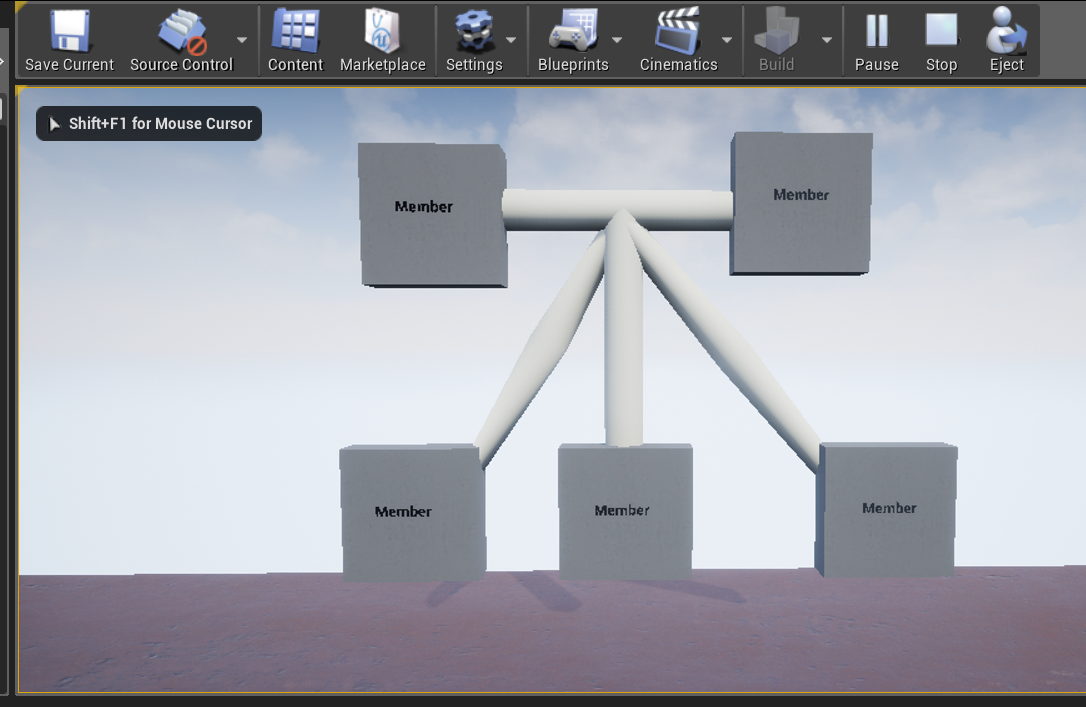
\includegraphics[height=7cm]{tree}
\newline

The floor that is seen in the picture has been used for debugging the overlapping and connections of the objects being displayed. This will be removed since users will be restricted to a specific view window. Light effect were added as a default setting, this will be removed since there is no need for the objects to display a shadow. 

I have also researched online for other open source blueprints that we could use for our project. I was able to find the spline pipeline through that, in addition to finding a way to toggle between desktop and VR. I have also been looking for blueprints to help manipulate data structures and how to display them to use in the future. In addition to blueprints, I found a lot of VR object building such as displaying and using a keyboard to type with in VR mode. I spent a lot of time exploring Unreal Engine and its features, in addition to finding ways of manipulating interactions. 

My next course of action would be to implement major user interaction with the objects. Upon selection, the object will be highlighted along with its relationships to other nodes (members of the family). I will also begin to implement a static menu bar window for the user to be able to call certain functions such as full or binary tree view, finding common ancestors, and to switch into VR mode.

Now that we have a working parser, we will also integrate that into Unreal Engine. Our parser has successfully worked as its own program and Unreal Engine also runs in C++ so the transition should hopefully be smooth. Once we are able to implement the parser into Unreal Engine, then we will be able to produce nodes with their given member's name. Because our parser also labels the relationship between each member, we will be able to create and display pipeline connections between each relating member according to their relationship with one another. 

Once we can successfully display a family tree, we will begin to implement the other features of our program. The algorithms for the binary tree and common ancestry will be programmed in C++ and then integrated into Unreal Engine. As mentioned before, each feature will be displayed via a button on the menu bar. In the case of the full binary tree option, this will initiate a new display but should still use the custom classes and interactions as the full ancestry tree. However, the common ancestor function should highlight the common ancestor as well as the pathway to the nodes that were selected. 

Once we are able to successfully run everything, we need to implement our final functionality: switching into VR. Luckily Unreal Engine has a built-in handler for VR. If a VR set is presented, then there will be an extra functionality available for the user to switch into VR. In VR mode, the display will generally be the same 3D objects as seen in the desktop version. Interactions will also be the same, so upon interacting with an object, the node will be highlighted along with their relationships to other members of the tree. The user will still be limited to how far they can zoom in and out, and how far they can scroll from the family tree. The largest difference would be how the user will access the other application's features. Instead of having a menu bar at the top of the screen, the user will be able to have a menu appear in their “hand”. VR remote buttons will be utilize to aid in scrolling, zooming, select, and right-click. Another difference is that when a user is searching for a common ancestor, a keyboard will appear on the screen for the user to type instead of having them remove their headset to manually use a keyboard.

The biggest and reoccurring problem I have had is working with Unreal Engine. Unreal Engine is focused on being a gaming software, so most of its features focuses on following certain “gaming rules”. This was apparent when even the most basic template form included a platform, light source objects, reflections objects, and shadow effects. For our very basic data display application, we didn't need these extra features. No one in my group is familiar with Unreal Engine either, so like any new software, we had to learn its numerous functions which hasn't been too difficult because the Unreal Engine documents provide a lot of information and tutorials. 

Initially, I was trying to create the objects on my own using basic assumptions, which worked well in the beginning in regard to rotating and changing sizes. However, my first small issue was attempting to create a texture pack and understanding how the blueprint functionality worked. This was easily solved with online tutorials and forums. This was helpful when I was attempting on creating a spline pipeline class and relationships between objects. Most of my issues have been small and annoying but were all existing problems that have been talked about. The Unreal Engine community has definitely been able to help me through most of my problems. Some issues were a bit harder to fix, such as the glitch with my spline pipeline, because many of the forums are unfortunately outdated. 
\end{singlespace}
\section{Le-Chuan Justin Chang}
\subsection{Introduction}
\begin{singlespace}
In general, the current status of the components listed are that they are designed, but not implemented. The largest roadblock is primarily time management, as the capstone tended to be prioritized last, since there were no set goals. This is an issue that hasn't yet been resolved, though a proposed solution is just to set personal, hard deadlines. The status, problems and design of each component assigned is listed below.
\end{singlespace}
\subsection{Algorithm}
\begin{singlespace}
The algorithm has been designed, but it has not been implemented, nor has it undergone extensive testing to prove its correctness. The objective for the algorithm is that it generates nodes with enough space between them so the amount of overlap for lines is minimal, and that there are no nodes that overlap. 

As stated before, the algorithm needs to be coded and tested. This will involve reading the data from the parser, then creating the algorithm from the design, then sending the design to the Unreal Engine visualization component for the data to be shown. There have not been any large roadblocks, aside from setting time aside to create and implement it. Overall, the algorithm is not as developed as it should be at this point in the term, though it is designed.

The current algorithm is designed as follows: The algorithm will ignore sibling relations, except with respect to placement for simplicity's sake. Before beginning, each parent pair is treated as a single node for placement purposes. The algorithm will start by iterating through the map that the data is stored in, and finding every pair of parents, or single parents if the spouse is unknown, that do not have parents. They will be labeled as root nodes, because they are the top of their tree. Each root will form trees that do not make contact with any of the other trees, though their nodes may appear in other trees. The algorithm will then go through each child attached to the root, attach their spouse, and then separate siblings by a fixed distance. Every subsequent child will separate their parent nodes as well, in order to maintain spacing. Finally, when the visualization occurs, there should be a line that connects nodes that are the same person if they are in a different location.
\end{singlespace}
\subsection{UI}
\begin{singlespace}
The UI has been designed, though there are two designs, and some consideration on which design should be implemented.\\
\newline
\includegraphics[height=5cm]{design1}
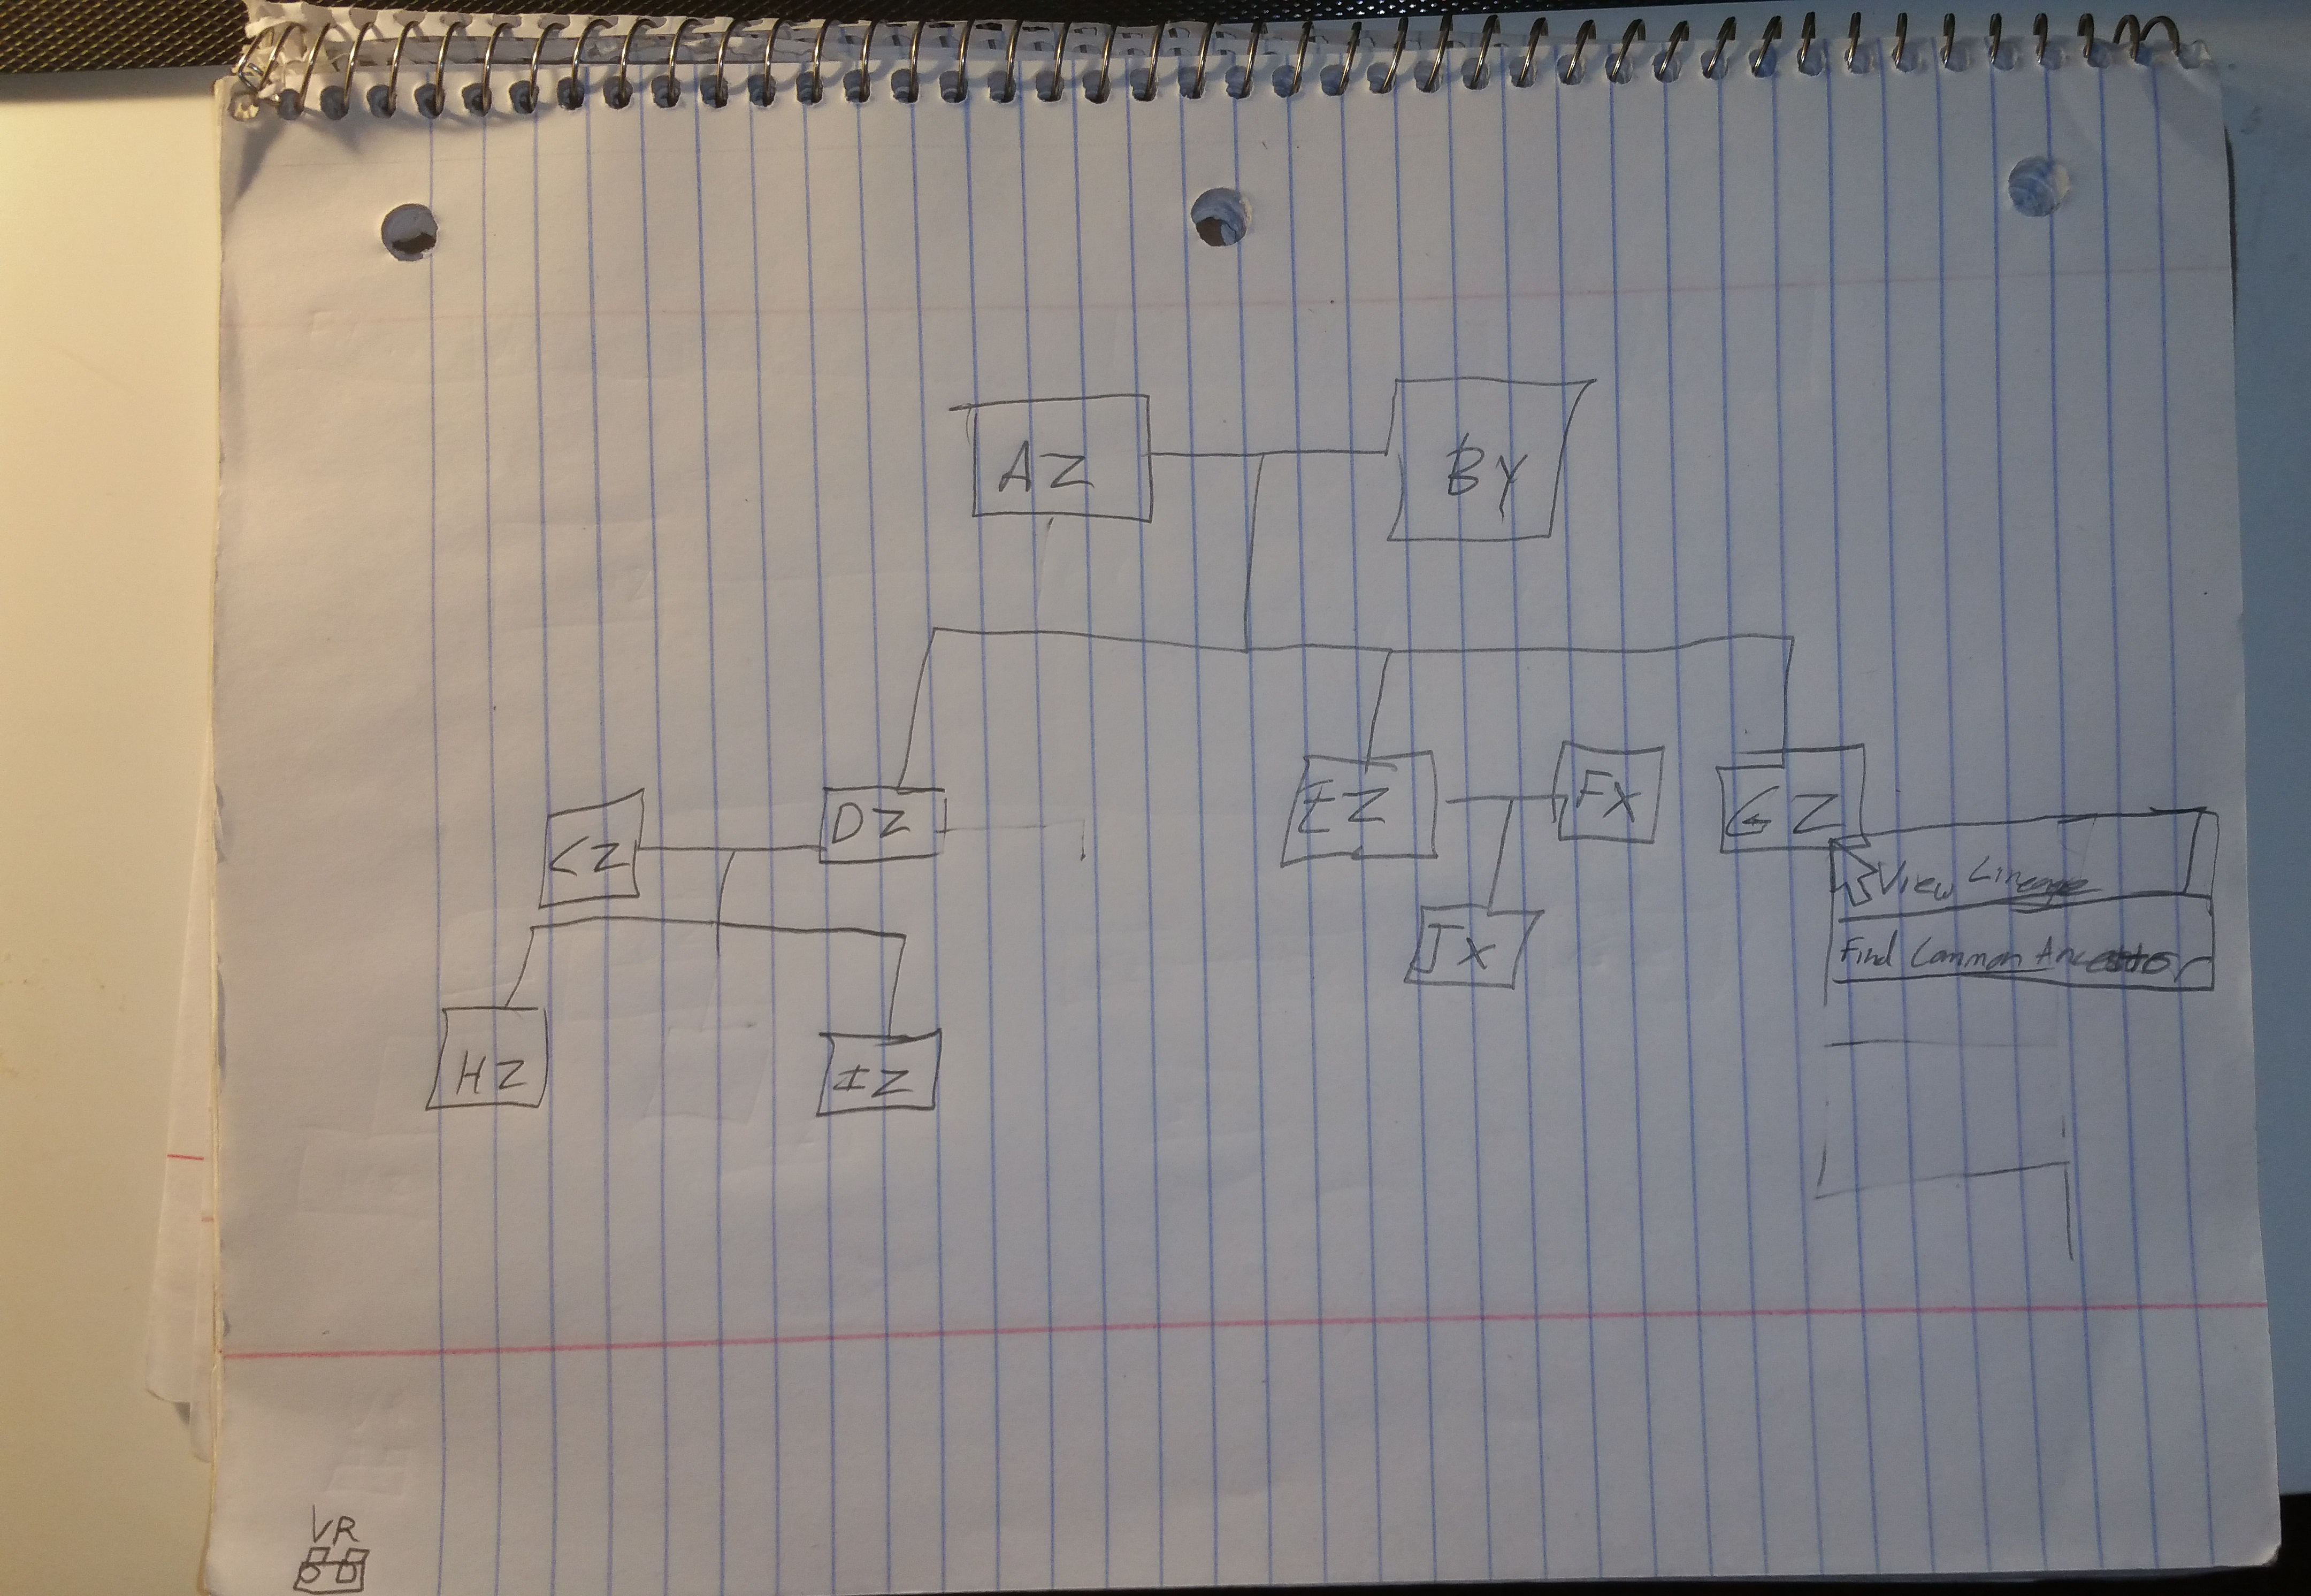
\includegraphics[height=5cm]{design2}
\newline
The first design, the left image, is more bulky, by virtue of having a permanently available menu always visible, as opposed to the second design having menus only appear when the user clicks on a node. The first design is currently favored, however, since while the first design has more always visible components, it is more intuitive precisely because of the menus being present. 


There is one additional concern with both of the designs. The nodes should appear as though they can be clicked on, because they all should double as buttons that allow the user to select the person that the node represents. This will likely require research on how to influence users to click objects that they aren't certain are interactable.

The current status the UI is at is implementation. The UI needs to be created using the UMG UI creator, then implemented. The primary concern to implementing the UI is attaching functionality to the buttons, for instance, changing the view style. Another potential concern would be implementing user selection. The intended functionality of user selection is that if they click a node, it should show the person as who the user has selected, write it on the first available “selected” bar, and highlight that node, and if they click the person again, all of the modifications should be removed. Selecting people would also automatically make them candidates for Lineage View and Nearest Common Ancestors. To remedy this, the UMG UI documentation should be consulted, and if that fails, the Unreal forums.
\end{singlespace}
\subsection{VR UI}
\begin{singlespace}
The VR UI has been designed, but the usability of the design has not been extensively tested. Fortunately, since the application's VR mode assumes that a VR controller is also in use, the UI is designed to be a menu attached to the fingers of a hand, which moves by the positional input from the controllers. Both hands serve the same purpose in terms of menus, but when selecting nodes, the controller that presses the button is also the one that selects the node. For instance, the user can activate find the nearest common ancestor with either hand, which will prompt both hands to switch to select a node mode. If the user points to two different nodes with both hands, but only wants to select the one that their right hand is pointing to, they simply press the select button on their right hand, and only the node that right hand is pointing at is selected. The user can then repeat the process to specify the other node with either hand.

The current status for this portion of the application is implementation, though it is further out than the other two portions, since the VR portions of the application has yet to be created. A possible solution to this particular roadblock would be to implement the portions that don't strictly need the rest of the system to be available, for instance, implementing the searches and views, or acquiring an asset for both of the user's arms.

The implementation of the VR UI should blend aspects of the normal UI with new aspects. In particular, the VR UI should keep the function implementation of the original UI, but instead of binding them to physical buttons on the menu, the functions should instead be bound to the buttons on the controller. Another addition to that menu is that the button menus should switch to a selection menu when necessary, for instance, when they user selects a menu option that requires node selection. Additionally, selection needs to be redone to accommodate for when the user points at a node. Finally, the hands that the user sees in VR mode must be created and designed to be of sufficient length, so that the user can adjust how far away the menu is from their face.
\end{singlespace}

\section{Conclusion }
\begin{singlespace}
Overall, the progress on the application has been poor over the current term. While research on how to perform each task has been done, and in many cases, completed, there is very little to show for it, as there has not been much implementation. There needs to be more hard deadlines set, and more strict leadership, so that time can be properly allocated for the development of the application.
\end{singlespace}

\end{document}